\documentclass[10pt,xcolor=pdflatex]{beamer}
\usepackage{newcent}
\usepackage[utf8]{inputenc}
\usepackage[czech]{babel}
\usepackage{hyperref}
\usepackage{fancyvrb}
\usepackage{graphicx}
\usepackage{textpos}
\usepackage{tikz}
\usepackage{textcomp}
\usepackage[export]{adjustbox}
\usepackage{float}
\usepackage{alltt}
\usepackage{hyperref}
\usetheme{FIT}

\newcommand{\myuv}[1]{\quotedblbase #1\textquotedblleft}
\def\uv#1{\quotedblbase#1\textquotedblleft}%

%%%%%%%%%%%%%%%%%%%%%%%%%%%%%%%%%%%%%%%%%%%%%%%%%%%%%%%%%%%%%%%%%%
\title[GJA 1]{Servlets, Java Server Pages}

\author[]{Jaroslav Dytrych}

\institute[]{Faculty of Information Technology
Brno University of Technology \\
Bo\v{z}et\v{e}chova 1/2. 612 66 Brno - Kr\'alovo Pole\\
dytrych@fit.vut.cz}

\date{18 September 2023}
%\date{\today}
%\date{} % bez data

%%%%%%%%%%%%%%%%%%%%%%%%%%%%%%%%%%%%%%%%%%%%%%%%%%%%%%%%%%%%%%%%%%

\begin{document}

\frame[plain]{\titlepage}

\begin{frame}\frametitle{Introduction}
  \begin{itemize}
    \item Lectures
      \begin{itemize}
        \item 2 hours a week
      \end{itemize}
    \item Points
      \begin{itemize}
        \item Midterm test -- 10
	    \item Team Project with defense -- 39 
	    \item[] (29 product, 5 documentation, 5 defense)
        \item Final exam -- 51 (10 points for the oral part)
      \end{itemize}
  \item Lower limits
  	\begin{itemize}
    	\item Team project -- 10
		\item Final exam -- 20
    \end{itemize}
  \item Projects
    	\begin{itemize}
    	\item Web (and mobile) application for 5 students
          \begin{itemize}
            \item Fewer students possible after consultation.
          \end{itemize}
    \end{itemize}	
  \end{itemize}
\end{frame}

\begin{frame}\frametitle{Course overview}
\begin{enumerate}
  \item Servlets, Java Server Pages
  \item Maven, Testing and JAX (Java API for XML)
  \item RMI (Remote Method Invocation) and JMS (Java Message Service)
  \item EJB (Enterprise Java Beans) and Java Server Faces
  \item PrimeFaces
  \item Spring
  \item[] Midterm test
  \item Lecture of an expert from practice
  \item JPA (Java Persistence API), Hibernate
  \item Google Web Toolkit
  \item Android basics
  \item Cloud
  \item Advanced Android
  \item[] Project defenses
\end{enumerate}
\end{frame}

\bluepage{Servlets}

\begin{frame}\frametitle{Content}
\begin{itemize}
	\item Servlet containers and application servers
	\item Introduction to servlets
	\item Deployment
	\item Servlet methods
	\item Servlet operations
	\item Annotations (declarative programming)
\end{itemize}
\end{frame}

\begin{frame}\frametitle{Java EE and Jakarta EE}
\begin{itemize}
	\item 1998 -- Sun started \emph{Java Professinoal Edition} project.
	\item 1999 -- Java 2 Platform Enterprise Edition (\emph{J2EE}) was born.
	\item 2006 -- J2EE was renamed to \emph{Java EE} or Java Platform Enterprise Edition.
	\item 2017 -- Oracle decided to give away the rights for Java EE to the Eclipse Foundation (the Java language is still owned by Oracle).
          \begin{itemize}
              \item  the Eclipse Foundation legally had to rename Java EE, because Oracle has the rights over the ``Java'' brand.
          \end{itemize}
	\item 2018 -- community voted for the new name and picked \emph{Jakarta EE}.
\end{itemize}
\end{frame}


\begin{frame}\frametitle{Servlet containers and application servers}
  \begin{itemize}
    \item Servlet containers
      \begin{itemize}
        \item Apache
          \begin{itemize}
            \item Tomcat \url{http://tomcat.apache.org/}
          \end{itemize}
        \item Eclipse Foundation
          \begin{itemize}
            \item Jetty \url{http://www.eclipse.org/jetty/}
          \end{itemize}
      \end{itemize}
 	\item Application servers
  	  \begin{itemize}
        \item Oracle
          \begin{itemize}
            \item GlassFish \url{https://javaee.github.io/glassfish/}
            \url{https://glassfish.org/}
          \end{itemize}
        \item Payara Services Ltd
          \begin{itemize}
            \item Payara \url{https://www.payara.fish/} -- drop in replacement for GlassFish
          \end{itemize}
        \item Red Hat
          \begin{itemize}
            \item WildFly (renamed from JBoss) \url{http://wildfly.org/}
          \end{itemize}
        \item IBM
          \begin{itemize}
            \item WebSphere Application Server \url{https://www.ibm.com/cloud/websphere-application-platform}
          \end{itemize}
      \end{itemize}
  \end{itemize}
\end{frame}


\begin{frame}\frametitle{CGI Scripts}
	\begin{itemize}
    	\item CGI stands for “Common Gateway Interface”.
        \item CGI script is an external program, which is called by the webserver. So the webserver is the mediator between the client and application.
        \item It is necessary to run a new instance for each request (it is stateless). \newline
    \end{itemize}
	\begin{minipage}{0.6\textwidth}
    \begin{enumerate}
      \item Client sends a request to server.
      \item Server starts a CGI script.
      \item Script computes a result for the server and quits.
      \item Server returns response to the client.
      \item Another client sends a request.
      \item Server starts the CGI script again.
    \end{enumerate} \hfill
    \end{minipage}
	 \begin{minipage}{0.3\textwidth}
    \begin{figure}[H]
    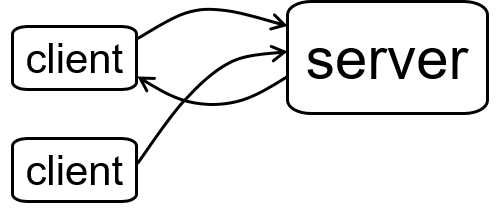
\includegraphics[scale=0.55]{img/obr1}
    \end{figure}
    \end{minipage} \hfill
\begin{tikzpicture}[remember picture,overlay]
    \node[xshift=-0.6cm,yshift=-1.3cm] at (current page.north east){%
    
\includegraphics[width=1cm]{img/lupa}};
\end{tikzpicture}
\end{frame}


\begin{frame}\frametitle{Servlets}
  \begin{itemize}
    \item A servlet is a small Java program that runs within a Web server. Simply said it is a Java class.
    \item From specification: For a servlet not hosted in a distributed environment (the default), the servlet container must use only one instance per servlet declaration. However, for a~servlet implementing the SingleThreadModel interface, the servlet container may instantiate multiple instances to handle a heavy request load and serialize requests to a~particular instance.\newline
  \end{itemize}
  \begin{minipage}{0.6\textwidth}
  \begin{enumerate}
   	\item Client sends a request to server.
    \item Server starts a servlet.
	\item Servlet computes a result for server and does not quit.
	\item Server returns response to client.
	\item Another client sends a request.
	\item Server calls the servlet again.
  \end{enumerate} \hfill
    \end{minipage}
	\begin{minipage}{0.3\textwidth}
    \begin{figure}[H]
    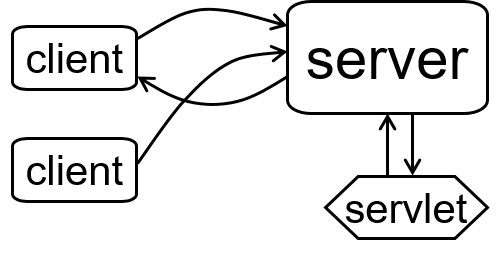
\includegraphics[scale=0.55]{img/obr2}
    \end{figure}
    \end{minipage} \hfill    
\begin{tikzpicture}[remember picture,overlay]
    \node[xshift=-0.6cm,yshift=-1.3cm] at (current page.north east){%
    
\includegraphics[width=1cm]{img/lupa}};
\end{tikzpicture}
\end{frame}


\begin{frame}\frametitle{Servlets vs. CGI scripts}
  \begin{itemize}
  	\item Advantages
    	\begin{itemize}
        	\item Running a servlet doesn’t require creating a separate process each time.
			\item A servlet stays in memory, so it doesn’t have to be reloaded each time.
			\item There is only one instance handling multiple requests, not a~separate instance for every request.
            \item It can keep context (session) in memory.
			\item Untrusted servlets can be run in a “sandbox”. \newline
        \end{itemize} 
       
	\item Disadvantage
	    \begin{itemize}
        	\item More complicated configuration.
        \end{itemize}	
  \end{itemize}
\begin{tikzpicture}[remember picture,overlay]
    \node[xshift=-0.6cm,yshift=-1.3cm] at (current page.north east){%
    
\includegraphics[width=1cm]{img/lupa}};
\end{tikzpicture}
\end{frame}


\begin{frame}[fragile]\frametitle{Servlets}
	\begin{itemize}
    	\item A servlet is any class that implements the \emph{javax.servlet.Servlet} or \emph{jakarta.servlet.Servlet} interface.
        \begin{itemize}
        	\item In practice, most servlets extends the \emph{javax.servlet.http.HttpServlet} or \emph{jakarta.servlet.http.HttpServlet} class (with built-in support for HTTP protocol).
			\item Some servlets extends 				\emph{javax.servlet.GenericServlet} or \emph{jakarta.servlet.GenericServlet} instead.
        \end{itemize}
        \item Servlets usually lack a main method, but must implement or override certain other methods.
	\end{itemize}
\begin{tikzpicture}[remember picture,overlay]
    \node[xshift=-0.6cm,yshift=-1.3cm] at (current page.north east){%
    
\includegraphics[width=1cm]{img/pozor}};
\end{tikzpicture}
\end{frame}
    
    
\begin{frame}[fragile]\frametitle{Important servlet methods}  
	\begin{itemize}
    	\item When a servlet is first started up, its~\emph{init(ServletConfig config)} method is called.
		  \begin{itemize}
        	\item \emph{init} should perform any necessary initializations.
			\item \emph{init} is called only once, and does not need to be thread-safe.
          \end{itemize}
        \item Every servlet request results in a call of \emph{service(ServletRequest request, ServletResponse response)}.
          \begin{itemize}
        	\item \emph{service} calls another method depending on the type of service requested -- e.g. \texttt{doGet()} or \texttt{doPost()}.
			\item Usually you would override the called methods of interest, not service itself.
			\item \emph{service} handles multiple simultaneous requests, so service and the methods it calls must be thread safe.
          \end{itemize}
        \item When the servlet is shut down, \emph{destroy()} is called.
          \begin{itemize}
        	\item \emph{destroy} is called only once, but must be thread safe (because other threads may still be running).
          \end{itemize}
    \end{itemize}
\begin{tikzpicture}[remember picture,overlay]
    \node[xshift=-0.6cm,yshift=-1.3cm] at (current page.north east){%
    
\includegraphics[width=0.8cm]{img/pozor}};
\end{tikzpicture}
\end{frame}


\begin{frame}\frametitle{Servlet deployment}
   	\begin{itemize}
       	\item Web archive
          \begin{itemize}
         	\item \texttt{ROOT/META-INF}
              \begin{itemize}
                \item Contains deployment descriptors.
                \item Typically contains \texttt{MANIFEST.MF}
               \end{itemize}
			 \item \texttt{ROOT/WEB-INF}
               \begin{itemize}
                 \item Can not be read by the client directly -- can be used for storing of database password and other secrets.
               \end{itemize}
          \end{itemize}
        \item Actual program
           \begin{itemize}
             \item \texttt{ROOT/WEB-INF/classes}
			 \item \texttt{ROOT/WEB-INF/libs}
           \end{itemize}
        \item Configuration file \texttt{web.xml} stored in \texttt{ROOT/WEB-INF}
          \begin{itemize}
            \item Contains
              \begin{itemize}
			    \item Filters
			    \item Init and context parameters
			    \item Servlet mapping
			    \item Error handlers
              \end{itemize}
        \item Alternatively configuration can be done by the annotations.
      \end{itemize}
    \end{itemize}
\begin{tikzpicture}[remember picture,overlay]
    \node[xshift=-0.6cm,yshift=-1.3cm] at (current page.north east){%
    
\includegraphics[width=1cm]{img/pozor}};
\end{tikzpicture}
\end{frame}


\begin{frame}[containsverbatim]\frametitle{Methods and configuration}  
	\begin{itemize}
    	\item Init param (for given servlet)
        {\scriptsize \begin{verbatim} 
// web.xml
<servlet>
    <servlet-name>controlServlet</servlet-name>
    <servlet-class>my.package.ControlServlet</servlet-class>
        <init-param>
            <param-name>myParam</param-name>
            <param-value>paramValue</param-value>
        </init-param>
</servlet>

// ControlServlet.java
  public void init(ServletConfig servletConfig) throws ServletException{
      this.myParam = servletConfig.getInitParameter("myParam");
  }
            \end{verbatim}
            }
        \item Context param (for whole application)
          {\scriptsize \begin{verbatim} 
<context-param>
    <param-name>myParam</param-name>
    <param-value>the value</param-value>
</context-param>

String myContextParam = request.getSession().getServletContext()
                        .getInitParameter("myParam");
\end{verbatim}}
 		\item Load on startup
          \begin{itemize}
            \item By default the servlet is loaded when first requested.
            \item Can be loaded immediately after server start or deployment:
            {\footnotesize \begin{verbatim} 
<load-on-startup>1</load-on-startup>
            \end{verbatim}
            }
          \end{itemize}
    \end{itemize}
\begin{tikzpicture}[remember picture,overlay]
    \node[xshift=-0.6cm,yshift=-1.3cm] at (current page.north east){%
    
\includegraphics[width=1cm]{img/oko}};
\end{tikzpicture}
\end{frame}


\begin{frame}[containsverbatim]\frametitle{Configuration} 
	\begin{itemize}
    	\item Filters
          \begin{itemize}
        	\item Mostly predefined filters from libraries.
            \item Used for various aspects like logging, security, etc.
            \item Security mostly handled otherwise.
          \end{itemize}
        
        \item[] \begin{scriptsize}\begin{verbatim} 
<filter>
    <filter-name>MyFilter</filter-name>
    <filter-class>my.package.MyFilter</filter-class>
</filter>
<filter-mapping>
    <filter-name>MyFilter</filter-name>
    <url-pattern>/*</url-pattern>
</filter-mapping>

public void doFilter(ServletRequest request, ServletResponse response,
        FilterChain filterChain) throws IOException, ServletException {
    log.warning("Log filter processed a " 
        + getFilterConfig().getInitParameter("logType")+ " request");
    filterChain.doFilter(request, response); // continue request processing
}
\end{verbatim}
 \end{scriptsize}
		\item Servlet mappings
        \item[] \begin{scriptsize} \begin{verbatim} 
<servlet>
    <servlet-name>comingsoon</servlet-name>
    <servlet-class>mysite.server.ComingSoonServlet</servlet-class>
</servlet>
<servlet-mapping>
    <servlet-name>comingsoon</servlet-name>
    <url-pattern>/*</url-pattern>
</servlet-mapping>
\end{verbatim} \end{scriptsize}
    \end{itemize}
\begin{tikzpicture}[remember picture,overlay]
    \node[xshift=-0.6cm,yshift=-1.3cm] at (current page.north east){%
    
\includegraphics[width=1cm]{img/lupa}};
\end{tikzpicture}
\end{frame}


\begin{frame}[containsverbatim]\frametitle{HTTP requests}
	\begin{itemize}
		\item The HTML \emph{} tag \texttt{form} has an attribute \emph{action}, whose value can be \emph{``get''} or \emph{``post''}.
        \item When a request is submitted from a Web page, it is almost always a \emph{GET} or a \emph{POST} request.
       	\item The \emph{``get''} action results in the form information being put after a  \emph{?} in the URL.
		  \begin{itemize}
            \item The \emph{\&} separates the various parameters.
            \item Example
            \item[] \url{http://www.google.com/search?hl=en&ie=UTF-8&oe=UTF-8&q=servlet}			  \item Only a limited amount of information can be sent this way.
          \end{itemize}
        \item \emph{``post''} can send large amounts of information.
    \end{itemize}
\begin{tikzpicture}[remember picture,overlay]
    \node[xshift=-0.6cm,yshift=-1.3cm] at (current page.north east){%
    
\includegraphics[width=1cm]{img/p}};
\end{tikzpicture}
\end{frame}

\begin{frame}[containsverbatim]\frametitle{Servlet methods}
  \begin{itemize}
	\item The \emph{service} method dispatches the following kinds of requests: \emph{DELETE}, \emph{GET}, \emph{HEAD}, \emph{OPTIONS}, \emph{POST}, \emph{PUT}, and \emph{TRACE}.
	  \begin{itemize}
	    \item A \emph{GET} request is dispatched to the \emph{doGet(HttpServletRequest~request, HttpServletResponse response)} method.
	    \item A \emph{POST} request is dispatched to the \emph{doPost(HttpServletRequest request, HttpServletResponse response)} method.
	    \item These are the two methods you will usually override.
	    \item \emph{doGet} and \emph{doPost} typically do the same thing, so usually you do the real work in one, and have the other just call it.
	    \item[] \begin{verbatim} 
public void doGet(HttpServletRequest request, 
                  HttpServletResponse response) {
    processRequest(request, response);
}
\end{verbatim} 
        \item Value of parameter can be acquired easily: \begin{verbatim} 
request.getParameter(name_of_parameter);
\end{verbatim} 
    \end{itemize}
  \end{itemize}
\begin{tikzpicture}[remember picture,overlay]
    \node[xshift=-0.6cm,yshift=-1.3cm] at (current page.north east){%
    
\includegraphics[width=1cm]{img/pozor}};
\end{tikzpicture}
\end{frame}


\begin{frame}[containsverbatim]\frametitle{A “Hello World servlet”}
	\begin{itemize}
    	\item[] \begin{footnotesize} \begin{verbatim} 
public class HelloServlet extends HttpServlet {
    public void doGet(HttpServletRequest request,
                      HttpServletResponse response)
                      throws ServletException, IOException {
        response.setContentType("text/html");
        PrintWriter out = response.getWriter();
        String docType = "<!DOCTYPE html>";
        out.println(docType +
                    "<html>\n" +
                    "<head><title>Hello</title></head>\n" +
                    "<body style=\"bgcolor:#FDF5E6;\">\n" +
                    "<h1>Hello World</h1>\n" +
                    "</body></html>");
     }
}
\end{verbatim} \end{footnotesize}
    \end{itemize}
  \begin{textblock}{6}(8.5,2.5)
    {\footnotesize Example servlet\_hello\_example}
  \end{textblock}
\end{frame}


\begin{frame}\frametitle{The superclass}
	\begin{itemize}
    	\item Every class must extend \emph{GenericServlet} or a subclass of \texttt{GenericServlet}.
		  \begin{itemize} 
            \item \emph{GenericServlet} is “protocol independent,” so you could write a servlet to process any protocol.
		    \item In practice, you almost always want to respond to an HTTP request, so you extend \emph{HttpServlet.}
		  \end{itemize}
		\item A subclass of \emph{HttpServlet} must override at least one method, usually one of \emph{doGet}, \emph{doPost}, \emph{doPut}, \emph{doDelete} and some of \emph{init}, \emph{destroy} and \emph{getServletInfo}.
    \end{itemize}
\begin{tikzpicture}[remember picture,overlay]
    \node[xshift=-0.6cm,yshift=-1.3cm] at (current page.north east){%
    
\includegraphics[width=1cm]{img/pozor}};
\end{tikzpicture}
\end{frame}


\begin{frame}[containsverbatim]\frametitle{The doGet method}
\begin{itemize}
    \item[] \begin{em}\begin{verbatim}
public void doGet(HttpServletRequest request,
            HttpServletResponse response)
            throws ServletException, IOException
\end{verbatim} \end{em}
    \item This method serves a \emph{GET} request.
    \item Input is in the \emph{HttpServletRequest} parameter.
    \item Output is via the \emph{HttpServletResponse} object, which we have named \emph{response}.
        \begin{itemize}
        	\item I/O in Java is very flexible but also quite complex, so this object acts as an “assistant”.
        \end{itemize}
	\item The method uses \emph{request} to get the information that was sent to it.
	\item The method does not return a value. Instead, it uses \emph{response} to get an I/O stream, and outputs its response.
	\item Since the method does I/O, it can throw an \emph{IOException}.
	\item Any other type of exception should be encapsulated as a~\emph{ServletException}.
	\item The \emph{doPost} method works \it{exactly} the same way.
\end{itemize}
\begin{tikzpicture}[remember picture,overlay]
    \node[xshift=-0.6cm,yshift=-1.3cm] at (current page.north east){%
    
\includegraphics[width=1cm]{img/pozor}};
\end{tikzpicture}
\end{frame}


\begin{frame}[containsverbatim]\frametitle{Input to the servlet}
\begin{itemize}
	\item A \emph{GET} request supplies parameters in the format
    \item[] \begin{footnotesize} \emph{URL?name=value\&name=value\&name=value} \end{footnotesize}
      \begin{itemize}
		\item Spaces in the parameter values are encoded by + signs or \texttt{\%20} (space is illegal in URL).
		\item Other special characters are encoded in hex; for example, an ampersand is represented by \emph{\%\texttt{$26$}}.
      \end{itemize}
    \item Input values are retrieved by parameter name (name of the form input). \begin{verbatim} 
request.getParameter(name_of_parameter);
\end{verbatim} 
	\item A \emph{POST} request supplies parameters in the same syntax, only it is in the “body” section of the request and it is therefore harder for the user to see it.
	\item Parameter names can occur more than once, with different values.
\end{itemize}
\end{frame}


\begin{frame}[containsverbatim]\frametitle{Getting the parameters}
\begin{itemize}
	\item Input parameters are retrieved via 
    \item[] \emph{HttpServletRequest} object \emph{request}.
	\item \emph{public Enumeration$\langle$String$\rangle$ getParameterNames()}
	  \begin{itemize}
    	\item Returns an \emph{Enumeration} of the parameter names.
		\item If there are no parameters, returns an empty \emph{Enumeration}.
      \end{itemize}
    \item \emph{public String getParameter(name)}
      \begin{itemize}
    	\item Returns the value of the parameter \emph{name} as a String.
		\item If the parameter doesn’t exist, returns \emph{null}.
		\item If name has multiple values, only the first is returned.
      \end{itemize}
	\item \emph{public String{\fontfamily{ptm}\selectfont []} getParameterValues(name)}
	\begin{itemize}
    	\item Returns an array of values of the parameter \emph{name}.
		\item If the parameter doesn’t exist, returns \emph{null}.
    \end{itemize}
    \end{itemize}
\end{frame}


\begin{frame}[containsverbatim]\frametitle{Example of input parameters}
\begin{itemize}
	\item[] \begin{footnotesize} \begin{verbatim}
public void doGet(HttpServletRequest request, 
                  HttpServletResponse response) {
    ... stuff omitted ...
    out.write("<H1>Hello");
    String names[] = request.getParameterValues("name");       
    if (names != null) {
        for (int i = 0; i < names.length; i++) {
            if {i == 0} {
              out.write(names[i]);
            } else {
              out.write(", " + names[i]);
            }
        }
    }
    out.write("!</H1>");
}
    \end{verbatim} \end{footnotesize}
\end{itemize}
\end{frame}


\begin{frame}[containsverbatim]\frametitle{Using the \textbf{HttpServletResponse}}
	\begin{itemize}
    	\item The second parameter of \emph{doGet} (or \emph{doPost}) is \emph{HttpServletResponse response}.
		\item Everything sent via the Web has a “MIME type” (RFC 2045 \url{https://www.ietf.org/rfc/rfc2045.txt}).
		\item The first thing we \textit{must} do with \emph{response} is set the \textit{MIME type} of our reply:
          \begin{itemize}
        	\item Following tells the client to interpret the page as HTML in UTF-8:
			\item[] \emph{response.setContentType("text/html;charset=UTF-8");}
          \end{itemize}
        \item Because we will be outputting character data, we will need a \emph{PrintWriter}, handily provided for us by the \emph{getWriter} method of \emph{response}:
        \item[] \emph{PrintWriter out = response.getWriter();}
        \item Now we’re ready to create the actual page to be returned.
    \end{itemize}
\begin{tikzpicture}[remember picture,overlay]
    \node[xshift=-0.6cm,yshift=-1.3cm] at (current page.north east){%
    
\includegraphics[width=1cm]{img/pozor}};
\end{tikzpicture}
\end{frame}


\begin{frame}[containsverbatim]\frametitle{Using the PrintWriter}
\begin{itemize}
	\item From here on, it’s just a matter of using our \emph{PrintWriter}, named \emph{out}, to produce the Web page.
	\item First we create a header string:
    \item[] \begin{footnotesize} \begin{verbatim}String docType = "<!DOCTYPE html>\n"; \end{verbatim} \end{footnotesize}
      \begin{itemize}
    	\item This line is technically required by the HTML specification.
		\item Browsers as IE can set particular page rendering mode. 
        \item Very important for HTML validators.
      \end{itemize}
    \item Then use the \emph{println} method of \emph{out} one or more times:
    \item[] \begin{footnotesize} \begin{verbatim}
out.println(docType +  
            "<html lang=\"en\">\n" +                    
            "<head> ... </body></html>");
\end{verbatim} \end{footnotesize}
\end{itemize}
  \begin{textblock}{5}(9.5,2.8)
    {\footnotesize Example servlet\_example}
  \end{textblock}
\end{frame}


\begin{frame}[containsverbatim]\frametitle{Typical servlet operations}
Servlet often serves as a mediator between the client and the enterprise application. Its typical operations are:
\begin{itemize}
	\item Input validation
	  \begin{itemize} 
    	\item Can be done also on client side.
      \end{itemize}
	\item Working with database
      \begin{itemize}
		\item Java persistence API
      \end{itemize}
	\item Uploading files
      \begin{itemize}
		\item Apache Commons
          \begin{itemize}
            \item Commons IO
            \item Commons FileUpload
          \end{itemize}
    	\item Can be handled directly in servlet 3.0 and above.
	  \end{itemize}
\end{itemize}
\end{frame}


\begin{frame}[containsverbatim]\frametitle{Commons FileUpload}
\begin{itemize}
	\item Depends on Commons IO.
	\item Contains classes for upload:
	\begin{itemize}
        \item \emph{DiskFileItemFactory}
        \item \emph{ServletFileUpload}
          \begin{itemize}
            \item Constructor \emph{ServletFileUpload(FileItemFactory fileItemFactory)}
            \item Method \emph{List$\langle$FileItem$\rangle$	parseRequest(HttpServletRequest request)}
          \end{itemize}
		\item \emph{FileItem}
		  \begin{itemize}
            \item \emph{String getFieldName()}
            \item \emph{String getContentType()}
            \item \emph{InputStream getInputStream()}
          \end{itemize}
    \end{itemize}
	\item Needs a repository when storing uploaded files to the file system (typically \texttt{/tmp}).
      \begin{itemize}
        \item Retrieved \emph{FileItem} is in \texttt{/tmp/}.
        \item When upload finished, we will move the file into the final location.
      \end{itemize}
	\item Can be loaded into \emph{ByteArray} when direct disk access is not available.
	  \begin{itemize} 
    	\item \emph{FileItemIterator}
		\item \emph{FileItemStream} (methods are similar as in \emph{FileItem})
	  \end{itemize}
\end{itemize}
\end{frame}


\begin{frame}[containsverbatim]\frametitle{Direct handling (from servlet 3.0)}
\begin{itemize}
	\item Request contains parts 
          \begin{itemize}
              \item  \texttt{Content-Type: multipart/form-data}
              \item \texttt{request.getParts()}
              \item \emph{jakarta.servlet.http.Part}
              \item \texttt{if (!filePart.\emph{getSubmittedFileName()}.isEmpty())}
              \item \emph{filePart.getInputStream()}
          \end{itemize}

	\item More properties:
	\begin{itemize}
        \item \emph{getSize()}
        \item \emph{	getContentType()}
    \end{itemize}
\end{itemize}
  \begin{textblock}{6}(8.3,3.8)
    {\footnotesize Example servlet\_upload\_example}
  \end{textblock}
\end{frame}

\bluepage{Annotations}

\begin{frame}[containsverbatim]\frametitle{Annotations}
\begin{itemize}
	\item Annotations enable a declarative style of programming.
	\item An annotation indicates that the declared element should be processed in some special way by a development tool, compiler, deployment tool, or during runtime.
	\item 3 Levels of Retention (\emph{RetentionPolicy}): 
      \begin{itemize}
        \item \emph{SOURCE} (processed by IDE -- e.g. NetBeans; discarded by compiler),
        \item \emph{CLASS} (default; processed during compilation and written to class file, not available in VM), 
        \item \emph{RUNTIME} (preserved in bytecode, available in runtime).
      \end{itemize}
    \item Any declaration can be annotated (package, class, interface, constructor, method, parameter, enumeration, variable, \ldots).
    \item Annotation can be also annotated (Meta Annotation).
\end{itemize}
\begin{tikzpicture}[remember picture,overlay]
    \node[xshift=-0.6cm,yshift=-1.3cm] at (current page.north east){%
    
\includegraphics[width=1cm]{img/pozor}};
\end{tikzpicture}
\end{frame}


\begin{frame}[containsverbatim]\frametitle{Annotation Declaration}
\begin{itemize}
	\item Types
	  \begin{itemize}
    	\item Normal Annotation (array of key -- value pairs)
		\item Single Member Annotation (one value)
		\item Marker Annotation (e.g. \texttt{@Override})
      \end{itemize}
	\item No exceptions from annotations.
	\item No inheritance.
	\item Methods return primitive types, \textit{String}, \textit{Class}, enum types, annotation types, or arrays of these types.
    \item Declared with \emph{@interface} (\texttt{@interface != interface}).
\end{itemize}
\begin{tikzpicture}[remember picture,overlay]
    \node[xshift=-0.6cm,yshift=-1.3cm] at (current page.north east){%
    
\includegraphics[width=1cm]{img/pozor}};
\end{tikzpicture}
\end{frame}


\begin{frame}[containsverbatim]\frametitle{Normal Annotation}
\begin{itemize}
	\item Normal Annotations takes multiple arguments. The syntax for these annotations provides the ability to pass in data for all the members defined in an annotation types.
	\item[] \begin{footnotesize} \begin{verbatim}
public @interface RequestForEnhancement {
    int id();
    String synopsis();
    String engineer() default "[unassigned]";
    String date() default "[unimplemented]";   
}
	\end{verbatim} \end{footnotesize}
    
    \item[] \begin{footnotesize} \begin{verbatim}
@RequestForEnhancement(
    id = 2868724,
    synopsis = "Provide time-travel functionality",
    engineer = "Mr. Doe",
    date     = "4/1/3017"     
) public static void travelThroughTime(Date destination) 
{ ... }
    \end{verbatim} \end{footnotesize}
\end{itemize}
\end{frame}

\begin{frame}[containsverbatim]\frametitle{Special annotations}
\begin{itemize}
	\item Single member
      \begin{itemize}
    	\item An annotation that only takes a single argument has a more compact syntax. You don't need to provide the member name.
        	\item[] \begin{footnotesize} \begin{verbatim}
public @interface Copyright {
    String value();
}

@Copyright("2006 Intelliware")
public class OscillationOverthruster { ... }
\end{verbatim} \end{footnotesize}
      \end{itemize}
    \item Marker
   	  \begin{itemize}
    	\item[] \begin{footnotesize} \begin{verbatim}
public @interface Preliminary { }

@Preliminary public class TimeTravel { ... }
\end{verbatim} \end{footnotesize}
      \end{itemize}
\end{itemize}
\end{frame}

\begin{frame}\frametitle{Built-in Annotations}
\begin{itemize}
	\item Java Annotations
      \begin{itemize}
        \item \emph{@Override} -- Indicates that a method declaration is intended to override a method declaration in a supertype (retention SOURCE). 
	    \item \emph{@Deprecated} -- A program element annotated is one that programmers are discouraged from using, typically because it is dangerous, or because a better alternative exists. Compilers warn when a deprecated program element is used or overridden in non-deprecated code (retention RUNTIME).
	    \item \emph{@SupressWarnings} -- Indicates that the named compiler warnings should be suppressed in the annotated element (retention SOURCE).
        \item \ldots
      \end{itemize}
\end{itemize}
\begin{tikzpicture}[remember picture,overlay]
    \node[xshift=-0.6cm,yshift=-1.3cm] at (current page.north east){%
    
\includegraphics[width=0.8cm]{img/pozor}};
\end{tikzpicture}
\end{frame}

\begin{frame}\frametitle{Meta-Annotations}
\begin{itemize}
	\item Meta-Annotations
      \begin{itemize}
        \item \emph{@Target} -- Indicates the kinds of program element to which an annotation type is applicable.
	    \item \emph{@Retention} -- Indicates how long annotations with the annotated type are to be retained.
        \item \emph{@Inherited} -- Indicates that an annotation type is automatically inherited. 
      \end{itemize}
\end{itemize}
\begin{tikzpicture}[remember picture,overlay]
    \node[xshift=-0.6cm,yshift=-1.3cm] at (current page.north east){%
    
\includegraphics[width=0.8cm]{img/pozor}};
\end{tikzpicture}
\end{frame}


\begin{frame}\frametitle{Meta-Annotation Examples}
\begin{itemize}
	\item[] @Target(value=METHOD)
	\item[] @Retention(value=SOURCE)
    \item[] public @interface Override \{\}
    \item[]
	\item[] @Target(value=\{TYPE,FIELD,METHOD,PARAMETER,CONSTRUCTOR, LOCAL\_VARIABLE\})
	\item[] @Retention(value=SOURCE)
	\item[] public @interface SuppressWarnings \{\ldots\}
\end{itemize}
\end{frame}


\begin{frame}[fragile]\frametitle{Meta-Annotation Inherited}
\begin{itemize}
    \small
	\item[] \texttt{@Inherited}
	\item[] \texttt{@Target(ElementType.TYPE)}
    \item[] \texttt{@Retention(RetentionPolicy.RUNTIME)}
    \item[] \texttt{public @interface InhAnType} \{ \ldots \}
	\item Annotation of this type will be inherited, so:
	\item[] \texttt{class First \{ \}}
	\item[] \texttt{@InhAnType}
	\item[] \texttt{class Second extends First \{ \}}
    \item[] \texttt{class Third extends Second \{ \}}
    \item[]
    \item[] \texttt{Class firC = new First().getClass();}
    \item[] \texttt{Class secC = new Second().getClass();}
    \item[] \texttt{Class thiC = new Third().getClass();}
    \item[] \texttt{System.out.println(firC.getAnnotation(InhAnType.class)); System.out.println(secC.getAnnotation(InhAnType.class)); System.out.println(thiC.getAnnotation(InhAnType.class));}
	\item[] Output:
	\item[] \texttt{ null}
	\item[] \texttt{ @InhAnType()}
	\item[] \texttt{ @InhAnType()}
	\normalsize
\end{itemize}
\begin{tikzpicture}[remember picture,overlay]
    \node[xshift=-0.6cm,yshift=-1.3cm] at (current page.north east){%
    
\includegraphics[width=0.8cm]{img/kompas}};
\end{tikzpicture}
\end{frame}


\begin{frame}\frametitle{Target values}
\begin{itemize}
	\item TYPE {\small -- class, interface (incl. annot. type), or enum declaration}
	\item TYPE\_PARAMETER
	\item FIELD
	\item METHOD
	\item PARAMETER
	\item CONSTRUCTOR
	\item LOCAL\_VARIABLE
	\item ANNOTATION\_TYPE
	\item PACKAGE
\end{itemize}
\end{frame}

\begin{frame}\frametitle{References}
	\begin{itemize}
    	\item Servlets
          \begin{itemize}
            \item \url{https://www.baeldung.com/java-enterprise-evolution}
        	\item \url{http://www.tutorialspoint.com/servlets/}
            \item \url{http://download.oracle.com/otndocs/jcp/servlet-3.0-fr-eval-oth-JSpec/}
          \end{itemize}
        \item Servlet configuration
          \begin{itemize}
            \item \url{https://jenkov.com/tutorials/java-servlets/web-xml.html}
            \item \url{https://cloud.google.com/appengine/docs/java/config/webxml}
          \end{itemize}
        \item{Java Annotations}
		  \begin{itemize}
        	\item \url{http://docs.oracle.com/javase/tutorial/java/annotations/}
            \item \url{https://docs.oracle.com/javase/7/docs/api/}
          \end{itemize}
    \end{itemize}
\end{frame}


\bluepage{Java Server Pages}

\begin{frame}\frametitle{Content}
	\begin{itemize}
    	\item Introduction
		\item Lifecycle
		\item Scriptlets
		\item Directives
		\item Expression Language
		\item Tags
    \end{itemize}
\end{frame}


\begin{frame}\frametitle{The problem with servlets}
	\begin{itemize}
        \item Servlet is common Java program running inside web or application server.
    	\item Servlets often contain request processing, business logic and code (\texttt{println}) to generate the HTML response.
		\item Servlet creators must be java programmers.
		\item Changing look/feel of a web app or upgrading to support new clients is hard if the GUI features are in the servlet.
		\item It is very hard to use web tools to develop an interface since the resulting HTML must still be manually hard-coded into the servlet.
    \end{itemize}
\end{frame}


\begin{frame}[containsverbatim]\frametitle{JavaServer Pages}
	\begin{itemize}
        \item JSP is written as ordinary HTML, with a little Java mixed in.
        \item The HTML is known as the template text.
	    \item The Java is enclosed in special tags, such as \verb;<%;\ldots \texttt{\%>}.
          \begin{itemize}
            \item JSP is similar to PHP, ASP, \ldots
          \end{itemize}
    	\item JSP (Java Server Pages) is an alternate way of creating servlets.
            \begin{itemize}
                \item JSP files must have the extension \texttt{.jsp}
				\item JSP is translated into a Java servlet, which is then compiled.
				\item Servlets are run in the usual way.
				\item The browser or other client sees only the resulting HTML, as usual.
            \end{itemize}
        \item Application server (AS) knows how to handle servlets and JSP pages.
		\item Support for EL (Expression Language), JSP tags, \ldots
        \item JSP can be combined with classic servlets in one application (e.g. JSP for mostly static pages, servlet for AJAX data).
    \end{itemize}
\begin{tikzpicture}[remember picture,overlay]
    \node[xshift=-0.6cm,yshift=-1.3cm] at (current page.north east){%
    
\includegraphics[width=1cm]{img/pozor}};
\end{tikzpicture}
\end{frame}


\begin{frame}[fragile]\frametitle{JSP Processing}
	\begin{itemize}
        \item JSP is typically compiled on first request. Then already compiled servlet is used. So first page load can be slower.
        \item All HTML is translated into \texttt{println()} in servlet.
    	\item [] \begin{center} 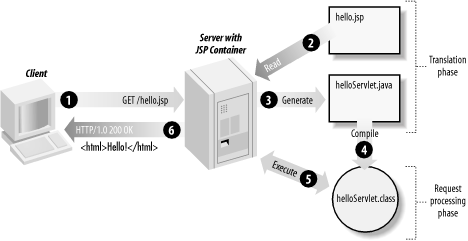
\includegraphics[scale=0.83]{img/obr3} \end{center}
    \end{itemize}
\begin{tikzpicture}[remember picture,overlay]
    \node[xshift=-0.6cm,yshift=-1.3cm] at (current page.north east){%
    
\includegraphics[width=1cm]{img/lupa}};
\end{tikzpicture}
\end{frame}


\begin{frame}\frametitle{JSP Advantages}
	\begin{itemize}
    	\item We are working with documents, not with Java classes.
        \item There can be only small pieces of Java code in the template text (look definition). This code can instantiate and use some classes with business logic. It is easier to change look and feel.
    \end{itemize}
\end{frame}


\begin{frame}[containsverbatim]\frametitle{JSP scripting elements}
	\begin{itemize}
    	\item There is more than one type of JSP “tag”, depending on what you want to do with the Java.
		\item \verb;<%=expression%>;
 		  \begin{itemize}
        	\item The expression is evaluated and the result is inserted into the HTML page.
          \end{itemize}
		\item \verb;<%code%>;
		  \begin{itemize}
        	\item The code is inserted into the servlet's \emph{service} method.
			\item This construction is called a \emph{scriptlet}.
          \end{itemize}
 		\item \verb;<%!declaration%>;
		  \begin{itemize}
        	\item The declarations are inserted into the servlet class, not into a~method.
		  \end{itemize}
    \end{itemize}
\begin{tikzpicture}[remember picture,overlay]
    \node[xshift=-0.6cm,yshift=-1.3cm] at (current page.north east){%
    
\includegraphics[width=1cm]{img/lupa}};
\end{tikzpicture}
\end{frame}


\begin{frame}[containsverbatim]\frametitle{Example JSP}
	\begin{itemize}
    	\item[] \begin{footnotesize} \begin{verbatim}
<HTML>
<BODY>
Hello! The time is now <%= new java.util.Date() %>
</BODY>
</HTML>
\end{verbatim} \end{footnotesize}
		\item[]
        \item[]
    	\item Notes:
		  \begin{itemize}
        	\item The \texttt{<\%=} \ldots \texttt{\%>} tag is used, because we are computing a~value and inserting it into the HTML.
			\item The fully qualified name \emph{java.util.Date} is used, instead of the short name \emph{Date} (use imports to handle this).
          \end{itemize}
    \end{itemize}
\end{frame}


\begin{frame}\frametitle{Implicit objects}
	\begin{itemize}
    	\item You can declare your own variables, as usual.
		\item JSP provides several predefined variables:
		  \begin{itemize}
        	\item \emph{request} --  The \texttt{HttpServletRequest} parameter.
			\item \emph{response} --  The \texttt{HttpServletResponse} parameter.
			\item \emph{out} --  A \texttt{JspWriter} (like a \texttt{PrintWriter}) used to send output to the client.
			\item \emph{config} -- Allows to pass the initialization data to a JSP page's servlet.
			\item \emph{page} -- Represents the current page that is used to call the methods defined by the translated servlet class.
			\item \emph{exception} -- Only for error pages.
			\item \emph{pageContext} --  The context for the JSP page itself that provides a single API to manage the various scoped attributes.
			\item \emph{session} --  The \texttt{HttpSession} associated with the request, or null if there is none.
			\item \emph{application} --  Allows to share the same information between the JSP page's servlet and any Web components with in the same application.
          \end{itemize}
    \end{itemize}
\begin{tikzpicture}[remember picture,overlay]
    \node[xshift=-0.6cm,yshift=-1.3cm] at (current page.north east){%
    
\includegraphics[width=1cm]{img/oko}};
\end{tikzpicture}
\end{frame}


\begin{frame}\frametitle{JSP scopes}
	\begin{itemize}
		\item Object scope in JSP is divided into four parts.
		\item \emph{page:}  can be accessed only from within the same page where it was created. JSP implicit objects \emph{out}, \emph{exception}, \emph{response}, \emph{pageContext}, \emph{config} and \emph{page} have ‘page’ scope.
		\item \emph{request:}  can be accessed from any page that serves that request. More than one page can serve a single request. Implicit object \emph{request} has the ‘request’ scope.
		\item \emph{session:}  is accessible from pages that belong to the same session from where it was created. Implicit object \emph{session} has the ‘session’ scope.
		\item \emph{application:} can be accessed from any pages across the application. Implicit object \emph{application} has the ‘application’ scope.
    \end{itemize}
\begin{tikzpicture}[remember picture,overlay]
    \node[xshift=-0.6cm,yshift=-1.3cm] at (current page.north east) \ldots \texttt{\%>} tags
		  \begin{itemize}
        	\item Scriptlets do not produce a value that is inserted directly into the HTML (as is done with \texttt{<\%=} \ldots \texttt{\%>)}.
			\item Scriptlets are Java code that may write into the HTML.
			\item Example:
            \item[] \begin{verbatim} 
<% String queryData = request.getQueryString();
out.println("Attached GET data: " + queryData); %>
\end{verbatim}
          \end{itemize}
        \item Scriptlets are inserted into the servlet \textit{exactly as written} (into the \emph{service} method), and are not compiled until the entire servlet is compiled.
    	  \begin{itemize}
        	\item Example (of wrong approach -- do not mix it so much):
            \item[] \begin{verbatim}
<% if (Math.random() < 0.5) { %>          
Have a <B>nice</B> day!<% } else { %>          
Have a <B>lousy</B> day!<% } %>
\end{verbatim}
          \end{itemize}
    \end{itemize}
\end{frame}


\begin{frame}[containsverbatim]\frametitle{Declarations}
	\begin{itemize}
    	\item Use \texttt{<\%!} \ldots \texttt{\%>} for declarations to be added to your servlet class, not to any particular method.
		  \begin{itemize}
        	\item \textbf{Caution}: Servlets are multithreaded, so nonlocal variables must be handled with extreme care.
			\item If declared with \texttt{<\% }\ldots  \texttt{\%>}, variables are local and OK.
			\item Data can also safely be put in the request or session objects.
          \end{itemize}
    	\item Example:
        \item[] \begin{verbatim}
<%! private int accessCount = 0; %>      
Accesses to page since server reboot: 
<%= ++accessCount %>
\end{verbatim}
        \item You can use \texttt{<\%!} \ldots \texttt{\%>} to declare methods as easily as to declare variables.
    \end{itemize}
\end{frame}


\begin{frame}[containsverbatim]\frametitle{Directives}
	\begin{itemize}
		\item Directives affects the servlet class itself.
        \item Directive is for JSP container and tells how to generate the servlet.
		\item A directive has the form:
          \begin{itemize}
        	\item[] \begin{verbatim}
<%@ directive attribute="value" %>\end{verbatim}
          \end{itemize}
        \item[] or
          \begin{itemize}
        	\item[] \begin{verbatim}
<%@ directive attribute1="value1"  
              attribute2="value2"
              ...
              attributeN="valueN" %>
\end{verbatim}
          \end{itemize}
    \item The most useful directives are:
      \begin{itemize}
    	\item \emph{page} -- lets you import packages, for example:
        \item[] \texttt{<\%@ page import="java.util.*" \%>}
    \item \emph{include} -- used to include a file into the JSP during the translation phase. It merges the content of other external files with the current JSP. Suitable e.g. for menu.
    \item \emph{taglib} -- tag library is a set of user-defined tags that implement custom behavior.
      \end{itemize}
    \end{itemize}
\begin{tikzpicture}[remember picture,overlay]
    \node[xshift=-0.6cm,yshift=-1.3cm] at (current page.north east){%
    
\includegraphics[width=1cm]{img/lupa}};
\end{tikzpicture}
\end{frame}


\begin{frame}\frametitle{The page directive}
	\begin{itemize}
    	\item Defines attributes that apply to an entire JSP page
          \begin{itemize}
            \begin{footnotesize}
            \item \emph{extends} -- Specifies the class from which the translated JSP will be inherited.
		    \item \emph{import} -- Specifies a comma-separated list of fully qualified type names and/or packages that will be used in the current JSP.
		    \item \emph{session} -- Specifies whether the page participates in a session.
		    \item \emph{buffer} -- Specifies the size of the output buffer used with the implicit object \texttt{out}.
		    \item \emph{autoFlush} -- When set to true (the default), this attribute indicates that the output buffer used with implicit object \texttt{out} should be flushed automatically when the buffer fills.
		    \item \emph{isThreadSafe} -- Specifies if the page is thread safe.
		    \item \emph{info} -- Specifies an information string that describes the page.
		    \item \emph{errorPage} -- Any exceptions in the current page that are not caught are sent to the error page for processing.
		    \item \emph{isErrorPage} -- Specifies if the current page is an error page that will be invoked in response to an error on another page.
		    \item \emph{contentType} -- Specifies the MIME type of the data in the response to the client.
		    \item \emph{pageEncoding} -- Specifies the page encoding of the current page.
            \end{footnotesize}
          \end{itemize}
    \end{itemize}
\end{frame}


\begin{frame}\frametitle{The include directive}
\begin{itemize}
	\item The \emph{include}\textbf{\textit{}} directive inserts another file into the file being parsed.
	  \begin{itemize}
		\item The included file is treated as just more JSP, hence it can include static HTML, scripting elements, actions and directives.
       \end{itemize}
	\item Syntax:  \texttt{<\%@ include file="\textbf{\textit{URL}}" \%>}
	  \begin{itemize}
    	\item The \emph{\textbf{\textit{URL}}} is treated as relative to the JSP page.
		\item If the \emph{\textbf{\textit{URL}}} begins with a slash, it is treated as relative to the home directory of the Web server.
      \end{itemize}
	\item The \emph{include} directive is especially useful for inserting things like navigation bars.
\end{itemize}
\end{frame}


\begin{frame}\frametitle{JSP comments}
	\begin{itemize}
    	\item Different from HTML comments.
		\item HTML comments are visible to the client.
          \begin{itemize}
        	\item[]
        	\item[] \texttt{<!-- an HTML comment -->}
            \item[]
          \end{itemize}
		\item JSP comments are used for documenting JSP code.
		\item JSP comments are not visible on client-side.
          \begin{itemize}
        	\item[]
        	\item[] \texttt{<\%-- a JSP comment --\%>}
            \item[]
          \end{itemize}        
    \end{itemize}
\begin{tikzpicture}[remember picture,overlay]
    \node[xshift=-0.6cm,yshift=-1.3cm] at (current page.north east){%
    
\includegraphics[width=1cm]{img/oko}};
\end{tikzpicture}
\end{frame}


\bluepage{JavaBeans}

\begin{frame}[containsverbatim]\frametitle{JavaBeans}
	\begin{itemize}
        \item A JavaBean is a reusable software component that can be~manipulated visually
in a builder tool.
        \item A JavaBean is a Java class written according to the JavaBeans API specifications.
        \item Following are the unique characteristics that distinguish a~JavaBean from other Java classes:
            \begin{itemize}
              \item It provides a default, no-argument constructor.
              \item It should be serializable and implement the \texttt{Serializable} interface.
              \item It may have a number of (private) properties which can be read or written.
              \item It may have a number of ``getter'' and ``setter'' methods for the properties.
              \item It may have a support for ``events'' as a simple communication metaphor which can be used to connect up beans.
            \end{itemize}
    \end{itemize}
\begin{tikzpicture}[remember picture,overlay]
    \node[xshift=-0.6cm,yshift=-1.3cm] at (current page.north east){%
    
\includegraphics[width=1cm]{img/lupa}};
\end{tikzpicture}
\end{frame}


\begin{frame}[containsverbatim]\frametitle{Getter and setter}
	\begin{itemize}
    	\item For each property (XXX) of component (bean), two methods getXXX and setXXX are implemented (``getter'' and ``setter''). Return type of the get method is the same as~the type of the parameter of the set method.
	      \begin{itemize}
            \item[] 
    	    \item[] \begin{verbatim}
public void setText(String text)
public String getText()
      \end{verbatim}
          \end{itemize}
    \item If the property is of type boolean, ``get'' is replaced by ``is''.
      \begin{itemize}
        \item[] 
    	\item[] \begin{verbatim}
public void setSelected(boolean b)
public boolean isSelected()
      \end{verbatim}
      \end{itemize}
    \end{itemize}
\end{frame}


\begin{frame}[containsverbatim]\frametitle{JavaBeans -- example}
	\begin{itemize}
    	\item[] \begin{footnotesize} \begin{verbatim}
public class Frog {
    private int jumps;
    private Color color;
    private boolean big;

    public int getJumps() {
        return jumps;
    }
    public void setJumps(int j) {
        jumps = j;
    }
    public Color getColor() {
        return color;
    }
    public void setColor(int c) {
        color = c;
    }
    public boolean isBig() {
        return big;
    }
    public void setBig(boolean b) {
        big = b;
    }
}	
	\end{verbatim}
    \end{footnotesize}
    \end{itemize}
\end{frame}


\begin{frame}[containsverbatim]\frametitle{JavaBean properties}
	\begin{itemize}
      \item Bound properties
		\begin{itemize}
		  \item Notify others of a property change event.
		  \item \emph{PropertyChangeEvent}
        \end{itemize}
      \item[] \begin{footnotesize} \begin{verbatim}
private final PropertyChangeSupport pcs =    
    new PropertyChangeSupport(this);
public void addPropertyChangeListener(PropertyChangeListener l) {
    this.pcs.addPropertyChangeListener(l); 
}
public void removePropertyChangeListener(PropertyChangeListener l) 
{
    this.pcs.removePropertyChangeListener(l); 
}
... 
this.pcs.firePropertyChange("name", oldName, newName);        
        \end{verbatim} \end{footnotesize}
		
      \item Vetoable properties
	    \begin{itemize}
		  \item \emph{VetoableChangeListener} (may throw \emph{PropertyVetoException})
        \end{itemize}
      \item[] \begin{footnotesize} \begin{verbatim}
public void setName(String newName) throws PropertyVetoException {  
    String oldName = this.name;  
    this.vcs.fireVetoableChange("name”, oldName, newName);  
    this.name = newName;  
    this.pcs.firePropertyChange("name", oldName, newName);      
}
\end{verbatim} \end{footnotesize}
	\end{itemize}
\begin{tikzpicture}[remember picture,overlay]
    \node[xshift=-0.6cm,yshift=-1.3cm] at (current page.north east){%
    
\includegraphics[width=1cm]{img/oko}};
\end{tikzpicture}
\end{frame}


\begin{frame}\frametitle{Expression Language}
	\begin{itemize}
    	\item Provides an important mechanism for enabling the presentation layer (web pages) to communicate with the application logic (managed beans).
		\item Used by both JavaServer Faces technology and JavaServer Pages (JSP) technology.
		\item Represents a union of the expression languages offered by JavaServer Faces technology and JSP technology.
    \end{itemize}
\end{frame}


\begin{frame}\frametitle{Expression language}
	\begin{itemize}
    	\item EL allows page authors to use simple expressions to dynamically access the data from JavaBeans components.
		\item EL is used for the following tasks:
          \begin{itemize}
			\item Dynamically read application data stored in JavaBeans components, various data structures, and implicit objects.
			\item Dynamically write data, such as user input from forms, to the JavaBeans components.
			\item Invoke arbitrary static and public methods.
			\item Dynamically perform arithmetic operations.
		  \end{itemize}
    \end{itemize}
\end{frame}


\begin{frame}[containsverbatim]\frametitle{Immediate and Deffered Evaluation Syntax}
	\begin{itemize}
    	\item Immediate Evaluation
		  \begin{itemize}
			\item All expressions written using the \verb;${}; syntax are evaluated immediately and value is returned on first page load.
            \item All immediately evaluated expressions are read only value expressions.
			\item It can be used only within template text or as the value of a~tag attribute that can accept runtime expressions.
			\item[] \verb;<fmt:formatNumber value="${sessionScope.cart.total}"/>;
            \item[] 
          \end{itemize}
    \item Deferred Evaluation
      \begin{itemize}
        \item Used mostly.
    	\item All expressions written using the \verb;#{}; syntax are evaluated as deferred.
		\item Expressions can be evaluated at other phases of a page lifecycle as defined by whatever technology is using the expression.
		\item[] \verb;<h:inputText id="name" value="#{customer.name}" />;
      \end{itemize}
    \end{itemize}
\begin{tikzpicture}[remember picture,overlay]
    \node[xshift=-0.6cm,yshift=-1.3cm] at (current page.north east){%
    
\includegraphics[width=1cm]{img/oko}};
\end{tikzpicture}
\end{frame}


\begin{frame}[containsverbatim]\frametitle{Value Expressions}
	\begin{itemize}
    	\item Rvalue expressions can read data but cannot write it.
		\item Lvalue expressions can both read and write data.
        \item Immediately evaluated expressions are always rvalue.
		\item Value expressions can refer to the following objects and their properties or attributes:
          \begin{itemize}
        	\item JavaBeans components
			\item Collections
			\item Java SE enumerated types
			\item Implicit objects
          \end{itemize}
      	\item \verb;.; or \verb;[]; notation \verb;${customer.name}; or \verb;${customer["name"]};
		\item An rvalue expression also refers directly to values that are not objects: \verb;${"literal"};, \verb;${customer.age + 20};, \verb;${true};, \verb;${57};
		\item Value expressions using the \verb;${}; delimiters can be used in static text or any standard or custom tag attribute that can accept an expression.
        \item \textbf{Properties of objects are automatically accessed through the getter and setter methods.}
    \end{itemize}
\begin{tikzpicture}[remember picture,overlay]
    \node[xshift=-0.6cm,yshift=-1.3cm] at (current page.north east){%
    
\includegraphics[width=1cm]{img/lupa}};
\end{tikzpicture}
\end{frame}


\begin{frame}[containsverbatim]\frametitle{Method expressions}
	\begin{itemize}
    	\item A method expression is used to invoke an arbitrary public method of a bean, which can return a result.
		\item Method expressions must always use the deferred evaluation syntax.
		\item Method expressions can use the \verb;.; and the \verb;[]; operators, \verb;#{object.method}; is equivalent to \verb;#{object["method"]};
		\item The EL offers support for parameterized method calls:
		  \begin{itemize}
            \item \verb;expr-a[expr-b](parameters);
 			\item[] \verb;#{userNumberBean[userNumber]('5')};
			\item \verb;expr-a.identifier-b(parameters);
			\item[] \verb;#{userNumberBean.userNumber('5')};
		  \end{itemize}
    \end{itemize}
\begin{tikzpicture}[remember picture,overlay]
    \node[xshift=-0.6cm,yshift=-1.3cm] at (current page.north east){%
    
\includegraphics[width=1cm]{img/lupa}};
\end{tikzpicture}
\end{frame}


\begin{frame}[containsverbatim]\frametitle{JSP tags}
	\begin{itemize}
		\item JSP tags have XML syntax.
		\item Supports Expression Language
        \begin{footnotesize}\begin{verbatim}
<%@ taglib prefix="c" uri="http://java.sun.com/jsp/jstl/core" %>
...
<c:set var="browser" value="${header['User-Agent']}"/>
<c:out value="${browser}"/>
        \end{verbatim}
        \end{footnotesize}
        \item Directive \emph{taglib} is used for import of tag libraries.
		\item JSTL -- JSP Standard Tag Library
		\item Separates logic from presentation layer.
		\item Java code goes into the bussines tier.
		\item Supports creating of new tags.
    \end{itemize}
\begin{tikzpicture}[remember picture,overlay]
    \node[xshift=-0.6cm,yshift=-1.3cm] at (current page.north east){%
    
\includegraphics[width=1cm]{img/oko}};
\end{tikzpicture}
\end{frame}


\begin{frame}[containsverbatim]\frametitle{JSP predefined tags}
	\begin{itemize}
        \item Predefined tags (JSP Actions) are available without any directive.
    	\item \verb;<jsp:include page="URL" />;
		  \begin{itemize}
			\item Inserts the indicated relative URL at execution time (not at compile time, like the include directive does).
			\item This is great for rapidly changing data.
		  \end{itemize}
        \item \verb;<jsp:forward page="URL" />;
        \item[] \verb;<jsp:forward page="<%= JavaExpression %>" />;
		  \begin{itemize}
            \item Forwarding a request to the another resource -- it can be a~JSP, static page such as html or Servlet or the (dynamically computed) JavaExpression resulting in a URL/JSP/servlet.
            \item Something as redirection.
		  \end{itemize}
        \item \begin{footnotesize}\verb;<jsp:getProperty name="bean" property="propertyName" />;\end{footnotesize}
          \begin{itemize}
        	\item Prints a particular feature of a given object.
           \end{itemize}
        \item \begin{footnotesize}\makebox[\linewidth][l]{\texttt{<jsp:setProperty name="bean"~property="prop"~param="paramName" />}}\end{footnotesize}
        \vspace{-0.35cm}
          \begin{itemize}
        	\item Setting the parameter value into property.
          \end{itemize}
    \end{itemize}
\end{frame}


\begin{frame}[containsverbatim]\frametitle{JSP useBean tag}
	\begin{itemize}
    	\item The \emph{useBean} (predefined) action tag is the most commonly used tag because of its powerful features.
		\item It allows a JSP to create an instance or receive an instance of a JavaBean.
		\item It is used for creating or instantiating a bean with a specific name and scope.
		\item Example:
		\item[] \verb;<jsp:useBean id="date" scope="session";
        \item[] \verb;class="java.util.Date" />;
        \item[] 
        \item[] \verb;<p>The date is <%= date %></p>;
    \end{itemize}
  \begin{textblock}{5}(10.0,2.4)
    {\footnotesize Example JSPExamples}
  \end{textblock}
\begin{tikzpicture}[remember picture,overlay]
    \node[xshift=-0.6cm,yshift=-1.3cm] at (current page.north east){%
    
\includegraphics[width=1cm]{img/lupa}};
\end{tikzpicture}
\end{frame}


\begin{frame}\frametitle{References}
	\begin{itemize}
    	\item JSP
        \begin{itemize}
        	\item \url{http://www.tutorialspoint.com/jsp/}
            \item \url{http://download.oracle.com/otndocs/jcp/7224-javabeans-1.01-fr-spec-oth-JSpec/}
            \item \url{http://docs.oracle.com/javaee/5/tutorial/doc/bnahq.html}
        \end{itemize}
    \end{itemize}
\end{frame}

\bluepage{Thank you for your attention!}


\end{document}
